\chapter{The Data Set}
\label{ch:data_collection}
\section{Overview}
Although we have discussed in detail the theoretical motivations for the W
physics program, as well as the machines producing the necessary collisions and
recording data produced from these collisions, we have not yet addressed the
form of the data set itself, and the substantial engineering it takes to extract
the signal of interest out of that data set.


The relative abundance of the $p + p \rightarrow W^\pm \rightarrow \mu^\pm +
\nu$ signal events is rather low, compared to the other interactions which may
take place when two protons collide. We must allow several hundred million
proton proton collisions to occur, before we have a high probability of
observing just one W-Boson event. 

We discussed in the previous chapter how careful triggering is employed in order
to ensure that any time this event does occur, it is recorded. This does not
guarantee that we \textit{only} record these events. Background events are still
recored much more frequently than signal events, even with the improved
triggering. The number of $W\rightarrow\mu$ events produced over the 2013 data
set number in the hundreds, while the total number of recorded events is
approximately 15 billion.

This leads to the substantial problem of fishing out the appropriate physics
events from the 15 billion event haystack. Why, I hear you ask, don't we just
have a detector which can record only the W-Boson events of interest?

Because, as a multipurpose spectrometer, PHENIX must be ready to take
all kinds of data, and satisfy many experimental requirements, in addition to
fitting a lot of functionality into a relatively tight budget, as is common for
federally funded research. Although this measurement would have been made
much simpler with a forward calorimeter, we can't simply build and install a
calorimeter the moment that an analysis would benefit from its presence.

So, instead, we must rely on our ingenuity and deep understanding of the data
set, to tease out the results we want to measure.

\section{Raw Data}

Any time a PHENIX trigger condition is satisfied, all of the information
recorded by the PHENIX spectrometer are read out from temporary on-detector
memory, and fed into a data stream that eventually is archived as a 'PHENIX Raw
Data File Format' or PRDFF. 

PRDFF data is hierarchical, first being organized by event-type, and
then organized by packet-type.  There are many event types - 'DATAEVENTS'
typically carry the information relevant to a physics analysis, whereas other
event-types carry very important QA information for determining the status of
the RHIC apparatus, the beam, polarization, and PHENIX performance.

Every packet has a header, which contains general information such as what the
packet contains, and in what order that packet was received. Every packet
recorded can be associated with a unique event-sequence number, which specifies
roughly the order in which the event owning the packet was received by the DAQ.
Within a given run number, an event-number is guaranteed to be unique. The
complexity of the packet is limited by the bandwidth available to move data off
PHENIX onto other storage, and the buffers/reconstruction ability of the front
end electronics modules built onto PHENIX subsystems. PHENIX archives data from
the DAQ at a rate of approximately 700 Megabytes per second - or one compact
disk.

Generally, raw PHENIX data is too complex to use straight-away, because minimal
to no reconstruction of physical properties for a certain event is done, due to
hardware limitations and time limitations - some of this raw data is often
directly used in triggering decisions, which must be made once every 106
nanoseconds or faster (the bunch crossing frequency).

The raw data collected from PHENIX undergoes a process called "Data Production",
where physical parameters are reconstructed from the simpler raw data. Raw data
could take any form - for example - which cathode strips were activated in an
event in the muon tracker, or, the number of photons counted in a
photomultiplier tube. This information is often combined with extensive survey
information about the geometry of a given detector, the known magnetic field in
a detector, to reconstruct quantities such as momentum, or deposited energy.

Once reconstruction has finished in a Data Production, the data are then
repackaged into ROOT files, often times internally structured into custom output
objects which are associated with a various detector. These output objects are
simply custom written C++ classes which have a serialization scheme, which have
libraries and dictionaries compiled that allow for them to be serialized into
ROOT's file format.

For the purposes of this analysis, all data has been reconstructed and
serialized into a specific type of output object called a 'picoDST' or even more
concisely, 'pDST'. This name, like many others in PHENIX has historical context:
DST stands for 'Data Summary Tape' hearkening back to the days when data was
stored primarily on magnetic tape (it is still archived on magnetic tape!), and
'pico' because of its relatively small disk-space requirement, compared to
'nanoDST' files or simply 'DST' files. I'm not making this up, I swear!

\section{Analysis Variables}

Even data reduced to the point of a pDST still is much more complicated and
comprehensive than what is needed for this analysis. The raw variables are
summarized on Tables \ref{tab:evt_variables},\ref{tab:mutr_variables},
\ref{tab:fvtx_variables} and \ref{tab:rpc_variables}. When Cartesian coordinates
are referenced, implicitly, the reference frame is the PHENIX Coordinate system
(Figure~\ref{fig:phenix_coordinate_system}).

\begin{table}[ht]
  \centering
  \begin{tabular}{l p{0.7\linewidth}}
    \toprule
      \textbf{Name} & \textbf{Description} \\
    \midrule
      Run\_Number & A unique number identifying a run in a RHIC fill for PHENIX \\
      Evt\_Number & A unique number within a single run identifying the approximate order an event was taken. \\
      Evt\_bbcZ & The event z-vertex calculated by the BBC \\
      triggerbit & The result of a bit-wise 'OR' applied to all 32-bit trigger bits which fired \\
    clockcross & The bunch number of the two colliding bunches $[0-119]$. Required to look up the spin polarization, along with Run\_Number \\
    \bottomrule
  \end{tabular}
  \caption{Variables characterizing events overall}
  \label{tab:evt_variables}
\end{table}

\begin{table}[ht]
  \centering
  \begin{tabular}{l p{0.7\linewidth}}
    \toprule
    \textbf{Name} & \textbf{(Unit) Description} \\
    \midrule
    Evt\_Nmu & The number of muon tracks reconstructed for a given event \\
    charge & ($\pm e$) The charge associated with a reconstructed muon track \\ 
    $p_z$ & (GeV) The z-momentum associated with the muon track \\
    $p$ & (GeV) The total momentum of a charged track \\
    $\chi^2$ & The result of the Kalman fitter reconstructing the track \\
    lastGap & The last gap in the Muon Tracker which was activated (there are 4) \\
    eta & The rapdity, $\eta$ of the track \\
    phi & (rad) The azimuthal position angle the track makes relative to the x-axis \\
    DG0 & (cm) A Track matching variable (matching between MuID and MuTR) associated with the MuID road, at MuID station 3. \\
    DDG0 & (degree)  The opening angle between the MuID track road, and the MuTr projection onto the MuID \\
    $xSta_i$ & (cm) The x-coordinate of the track at Station i,  $i\in{1,2,3}$ of the MuTr \\
    $ySta_i$ & (cm) The y-coordinate of the track at Station i, $i\in{1,2,3}$ of the MuTr \\

    $\phi_i$ & (rad) The angle the track makes with Station i, $i\in{1,2,3}$, i.e.: $\phi_i = tan^{-1}\left({{x_1}\over{y_i}}\right)$ \\
    $\theta$ & (rad) Azimuthal angle of track, $tan^{-1}\left({p_T \over p_z}\right)$ \\
    $DCA_z$ & (cm) Distance of closest approach between the z-vertex positions extracted by projecting the MuTR track z-vertex back to the BBC z-vertex \\
    $DCA_r$ & (cm) Distance of closest approach between the track and beam axis \\ 
    \bottomrule
  \end{tabular}
  \caption{
    Muon tracker variables. Generally, this data set is indexed on a subevent 
    level, where one event will contain all reconstructed muon tracks seen for 
    that event.
  }
  \label{tab:mutr_variables}
\end{table}

\begin{figure}[ht]
  \centering
  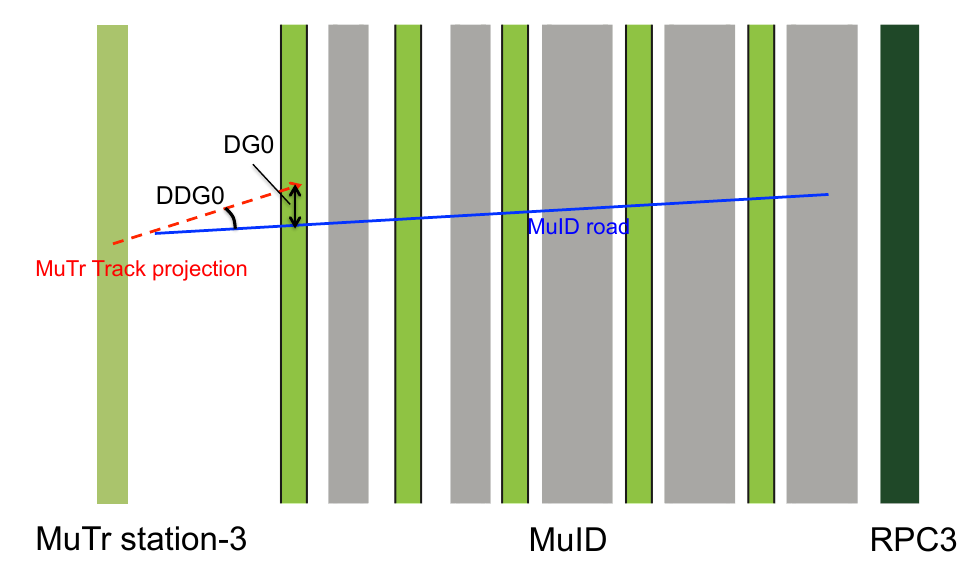
\includegraphics[width=0.7\linewidth]{./figures/dg0_ddg0.png}
  \caption{
    A schematic representation of the matching variables, DG0 and DDG0 at
    the intersection between the Muon Tracker and Muon 
    Identifier~\cite{Oide2012}
  }
  \label{fig:dg0_ddg0}
\end{figure}

\begin{table}[ht]
  \centering
  \begin{tabular}{l p{0.7\linewidth}}
    \toprule
    \textbf{Name} & \textbf{Description} \\
    \midrule
    $fvtx_{d\phi}$ & The $\phi$ residual between MuTR track and FVTX track \\
    $fvtx_{d\theta}$ & The $\theta$ residual between the MuTR track and FVTX track \\
    $fvtx_{dr}$ & The radial residual between the MuTR track and the FVTX track \\
    $fvtx_{conebits}$ & The number of FVTX clusters inside a cone around the track defined by: $0.04 rad < dR < 0.52 rad$ where $dR = \sqrt{{d\eta}^2+{d\phi}^2}$\\
    \bottomrule
  \end{tabular}
  \caption{A summary of the variables reconstructed from FVTX raw data~\cite{Meles2015}.}
  \label{tab:fvtx_variables}
\end{table}

\begin{table}[ht]
  \centering
  \begin{tabular}{l p{0.7\linewidth}}
    \toprule
    \textbf{Name} & \textbf{Description} \\
    \midrule
    RpcMatchSt1 & Distance of closest approach between projected MuTR track onto the RPC 1 and the closest hit cluster on RPC 1\\
    RpcMatchSt3 & Distance of closest approach between projected MuTR track onto the RPC 3 and the closest hit cluster on RPC 3\\
    \bottomrule
  \end{tabular}
  \caption{RPC Track matching variables}
  \label{tab:rpc_variables}
\end{table}

\begin{figure}
  \centering
  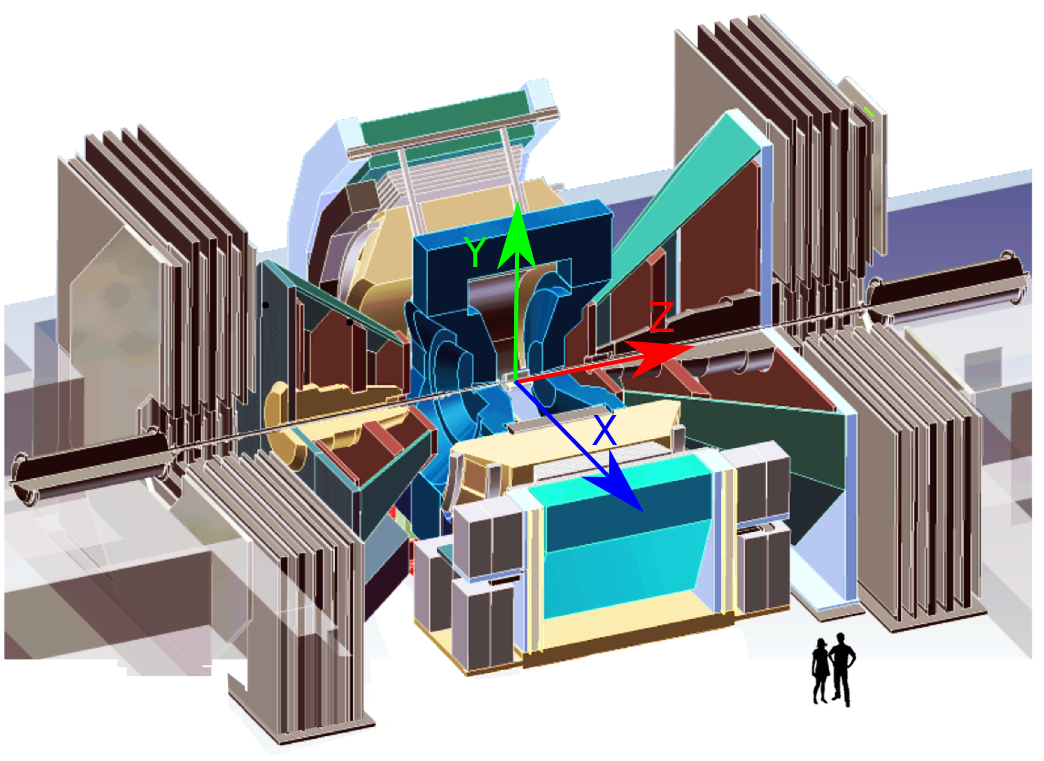
\includegraphics[width=0.8\linewidth]{./figures/phenix_coordinate_system.png}
  \caption{
    The PHENIX coordinate system is shown (RGB arrows) at the center of the
    nominal interaction point within PHENIX, the origin, in this quarter-cutaway
    drawing. The small black figures are actually miniaturized human beings, the
    PHENIX detector is very small - this is a full scale drawing of 
    PHENIX~\cite{WebPHENIXDrawings}
  }
  \label{fig:phenix_coordinate_system}

\end{figure}


\begin{figure}
  \centering
  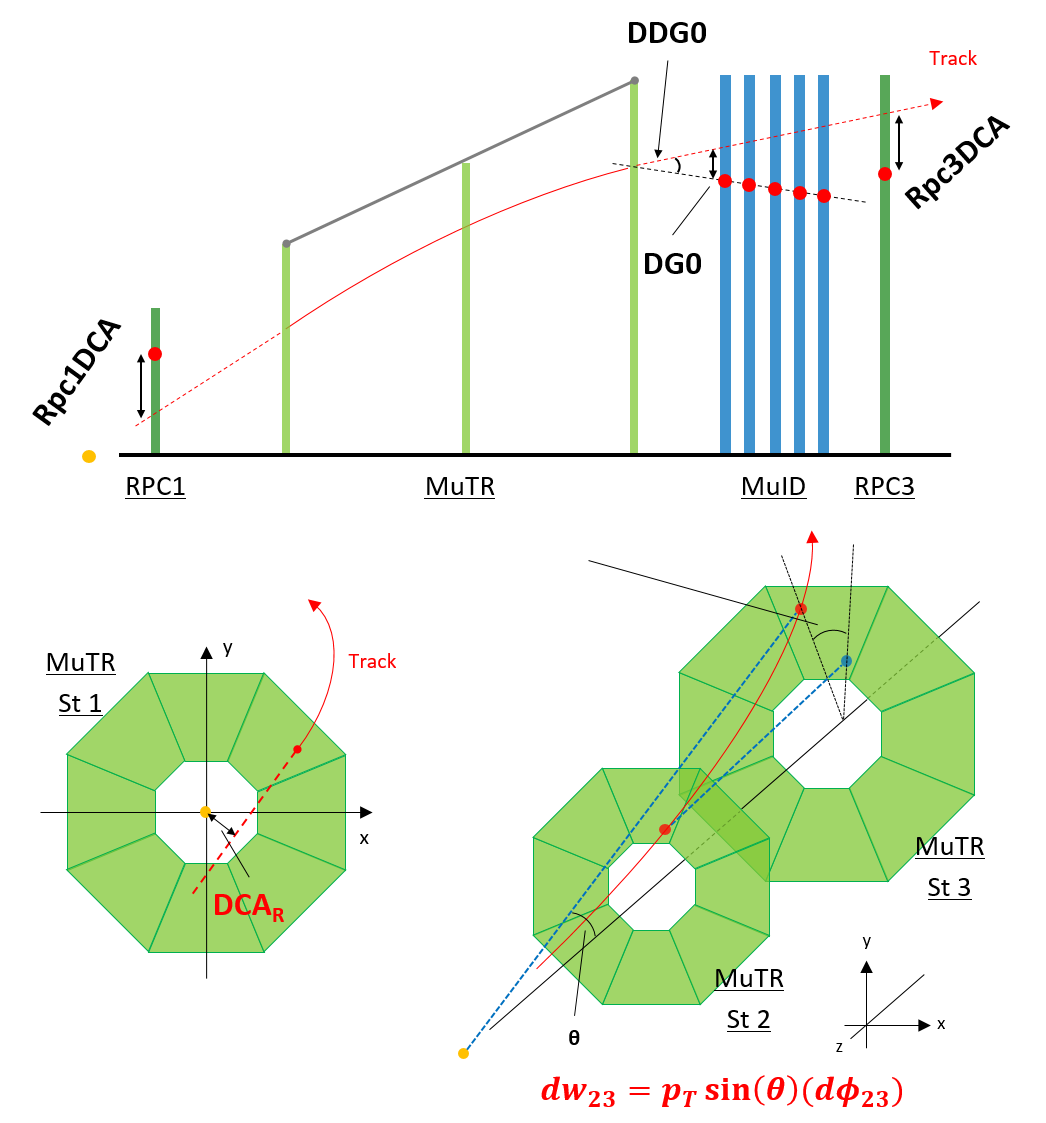
\includegraphics[width=0.8\linewidth]{./figures/kinematic_variables_schematic.png}
  \caption{
    A nice summary of discriminating kinematic variables reproduced with
    permission from Dr. Chong Kim.
  }

\end{figure}

\clearpage
\section{Delete this?}

In this chapter, we will discuss the process of cleaning our data set, the goal
of which is to get rid of background data, while keeping any event that could
possibly contribute to the $W\rightarrow\mu$ signal. This cleaning is done in
three stages. The first stage concerns applying a simple basic cut to our data
set to remove events which are kinematically forbidden from having $W$ boson
parent particles, this is called the "Basic Cut".

After this, we label data with $W_{ness}$, which is an event's likelihood for
coming from a $W$ boson decay. Although this is part of data cleaning, since
$W_{ness}$ is an important parameter in the analysis, it is discussed in
Section~\ref{ssec:likelihood}.

Finally, we must estimate the overall yield of $\mu$ resulting from the various
proton helicity combinations, and the signal to background ratio characterizing
that yield. Again, since this is also an important part of the physics, it is
discussed in Section ~\ref{ssec:sbr}.

\section{Analysis Variables and the Basic Cut}

A brief summary of the kinematic variables used later in the analysis is given
in Table~\ref{tab:basic_cut}. In addition four sets of RPC cluster variables exist
which are being used as main RPC variables. These variables contain
projections from either vertex, Station 1, 3 or the MuID road to the
corresponding z positions of the RPCs based on the tracks in the PHMuoTracksOut
node and are directly taken over from the RpcMuoTracks node in the dsts:

\begin{itemize}
\item newsngmuons$\rightarrow$Branch("RpcMatchVtx",0,"Rpc3dca[\_RecoTracks]/F:\\Rpc3time[\_RecoTracks]/F:Rpc3x[\_RecoTracks]/F:Rpc3y[\_RecoTracks]/F:\\Rpc1dca[\_RecoTracks]/F:Rpc1time[\_RecoTracks]/F:Rpc1x[\_RecoTracks/F:\\Rpc1y[\_RecoTracks]/F");
\item newsngmuons$\rightarrow$Branch("RpcMatchSt1",0,"Rpc3dca[\_RecoTracks]/F:\\Rpc3time[\_RecoTracks]/F:Rpc3x[\_RecoTracks]/F:Rpc3y[\_RecoTracks]/F:\\Rpc1dca[\_RecoTracks]/F:Rpc1time[\_RecoTracks]/F:Rpc1x[\_RecoTracks]/F:\\Rpc1y[\_RecoTracks]/F");
\item newsngmuons$\rightarrow$Branch("RpcMatchSt3",0,"Rpc3dca[\_RecoTracks]/F:\\Rpc3time[\_RecoTracks]/F:Rpc3x[\_RecoTracks]/F:Rpc3y[\_RecoTracks]/F:\\Rpc1dca[\_RecoTracks]/F:Rpc1time[\_RecoTracks]/F:Rpc1x[\_RecoTracks]/F:\\Rpc1y[\_RecoTracks]/F");
\item newsngmuons$\rightarrow$Branch("RpcMatchMuID",0,"Rpc3dca[\_RecoTracks]/F:\\Rpc3time[\_RecoTracks]/F:Rpc3x[\_RecoTracks]/F:Rpc3y[\_RecoTracks]/F:\\Rpc1dca[\_RecoTracks]/F:Rpc1time[\_RecoTracks]/F:Rpc1x[\_RecoTracks]/F:\\Rpc1y[\_RecoTracks]/F");
\end{itemize}

\begin{table}
  \centering
  \begin{tabular}{ p{0.2\linewidth} p{0.7\linewidth} }
    \toprule
    \textbf{Variable} & \textbf{Definition} \\
    \midrule 
    $\eta$               & Pseudorapidity, used in secondary likelihood cuts \\
    $\chi^{2}_{track}$   & Standard chi2 of $\mu$ track Kalman fitter\\
    $DG0$,$DDG0$         & Roads generated in MUID+MuTr planes. $DG0$ is distance between first gap road and track. $DDG0$ is opening angle between road and track. \\
    $DCA_r$,$DCA_Z$      & Distance of closest approach between $\mu$ track and beam axis ($DCA_r$). $DCA_Z$ is the distance between the track's intersection with PHENIX's z-axis and the event vertex. \\
    $RpcDca_{1,3}$       & Distance between extrapolated track at RPC 1 or 3, and hit cluster at RPC 1 or 3. \\
    $dw_{23}$            & Reduced azimuthal bending angle of track. $dw_{23} = p_T sin(\theta)(\phi_2-\phi_3)$ \\
  \begin{tabular}[x]{@{}c@{}@{}}$fvtx\_d\theta$ \\$fvtx\_d\phi$\\$fvtx\_dr$\end{tabular}& FVTX matched track matching residuals for $\phi, \theta,dr$.\\
    \bottomrule
  \end{tabular}
  \caption{ Summary of engineered features from the data set used in this analysis. }
  \label{tab:kinematic_varaibles_summary}
\end{table}

For the moment the timing and DCA distributions we use are those matching from
station 1 for RPC1 and from station3 for RPC3.  In addition, in order to improve
the background rejection in the FVTX acceptance, for this analysis several new
variables are added in relation to the FVTX-MuTr matching which were directly
taken over from the corresponding methods  in the PHMuoTracksOut node. Those are
fvtx\_dr, fvtx\_d$\phi$ and fvtx\_d$\theta$ which compare the FVTX tracklets
radial position, azimuthal and polar angles with those of the MuTr as an
extrapolated z position between the two.  Another FVTX related addition is the
FVTX hit multiplicity within a cone of \textcolor{red}{INPUT RANGE HERE}  around
the projected track. This varible will henceforth be called FVTX\_cone.  

The "Basic Cut" is defined:
\begin{table}
	\begin{centering}
		\begin{tabular}{l c c}
			\toprule
			\textbf{Variable} & \textbf{Lower Bound} & \textbf{Upper Bound} \\
			\midrule
			MuID lastGap & * & Gap 4 \\ 
			$\chi^2$ & 0 & 20 \\
			$DG0$ & 0 & 20 \\
			$DDG0$ & 0 & 9 \\
			$\mu$ candidate & * & 1 \\
			\bottomrule
		\end{tabular}
		\caption{ The Basic Cuts used in the Run 13 analysis. lastGap refers to the
			last gap in the MUID which saw a $\mu$ candidate event. The fourth gap is
			the furthest penetration possible, therefore suggesting a high energy muon.
		Other parameters are described in table~\ref{tab:kinematic_varaibles_summary}}
		\label{tab:basic_cut}
	\end{centering}
\end{table}



In this W analysis one is interested in removing most lower momentum particles
which originate predominantly from background processes while keeping most of
the W decay muons. With the above cuts, we aim to reduce part of the fake muons
background assuring a good muon track reconstruction ($DG0$,$DDG0$ and $\chi^2$
cuts) and selecting tracks with momentum smaller than the maximum possible
physical energy. After applying these basic cuts, the background will be further
reduced via a likelihood method, described in Section~\ref{ssec:likelihood}, where
background and signal features will be studied in detailed.

The correlations between the several cut variables are shown in
Fig.~\ref{fig:kinematic_var_correlations} for data and for the W-si The only
exception is the correlation between the vertex extrapolated variables DCA\_z
and DCA\_r and the FVTX related matching variables. This is not entirely
unexpected as both should be sensitive to the amount of multiple scattering in
the central magnet yoke and initial shielding.

\section{Feature Engineering}
\subsection{Discriminating Kinematic Variables}
\subsection{Simulations}
